\documentclass[a4paper]{article}
\usepackage[latin1]{inputenc}
\usepackage{geometry}
\usepackage{amssymb}
\usepackage{framed}
\usepackage{amsmath}
\usepackage{graphicx}
\usepackage{booktabs}
\usepackage{subcaption}

\setlength{\parindent}{0pt}
\setlength{\parskip}{3ex}

\begin{document}

\begin{center}
  {\large Artificial Neural Networks and Deep Architectures, DD2437}\\
  \vspace{7mm}
  {\huge Short report on lab assignment 4\\[1ex]}
  {\Large Restricted Boltzmann Machines and Deep Belief Networks}\\
  \vspace{8mm}  
  {\Large Hilding Wollbo\\}
  \vspace{4mm}
  {\large October 7, 2020\\}
\end{center}

%\begin{framed}
%Please be aware of the constraints for this document. The main intention here is that you learn how to select and organise the most relevant information into a concise and coherent report. The upper limit for the number of pages is 6 with fonts and margins comparable to those in this template and no appendices are allowed. \\
%These short reports should be submitted to Canvas by the authors as a team before the lab presentation is made. To claim bonus points the authors should uploaded their short report a day before the bonus point deadline. The report can serve as a support for your lab presentation, though you may put emphasis on different aspects in your oral demonstration in the lab.
%Below you find some extra instructions in italics. Please remove them and use normal font for your text.
%\end{framed}

\section{Main objectives and scope of the assignment}
In this assignment we study Restricted Boltzmann Machines and Deep Belief Networks for classifying and generating images from the MNIST dataset. The RBM was trained using the Contrastive Divergence algorithm, a variant of Gibbs sampling. The DBN was trained using layer-wise pre-training and the wake-sleep algorithm for fine-tuning.
\section{Method}
The tasks were implemented in Python using numpy for data manipulation in matrices as well as matplotlib for producing the graphics and plots.
\section{Restricted Boltzmann Machine}
This RBM was trained using Gibbs sampling, where the conditional distributions $p(v\vert\mathbf{h}), p(v\vert\mathbf{h})$ are estimated iteratively using simultaneous sampling of the visible units given the hidden units and the hidden units given the visible units. This procedure can be run for an arbitrary number of steps, but in this task only 1 iteration was run per parameter update. Gibbs sampling is a Markov Chain Monte Carlo method, where each produced sample is conditionally independent given its neighbouring states. This sampling procedure thus produces a Markov chain, and given the attributes of invariance, periodicity and irreducibility, will converge to the true distribution of the samples. This means that using iterated sampling of the conditional probabilities does not change the joint probability between hidden and visible units, and we can infer that these probability distributions will converge given infinite repeated steps of Gibbs sampling. \\
In the first task, RBMs were constructed with $784 = 28^2$ visible units, with 200, 350 and 500 hidden units respectively. A learning rate of 0.01 was used, and a momentum term of 0.5 was added to facilitate convergence. The batch size was chosen as 20, and the training process was run for a total of 30 000 iterations, corresponding to 10 full epochs. This yielded the results in Figure \ref{fig:rbm}. An example of the weights of the network as training progresses is shown in Figure \ref{fig:receptive}. Few of these weights clearly map directly to a specific digit, instead showing a mixture of different digits.

\begin{figure}[ht]
   \centering
   \includegraphics[width=\linewidth]{figures/rbm.pdf}
   \caption{The reconstruction error over iterations for different architectures}
   \label{fig:rbm}
\end{figure}

\begin{figure}[ht]
  \begin{subfigure}[b]{0.3\textwidth}
   \centering
   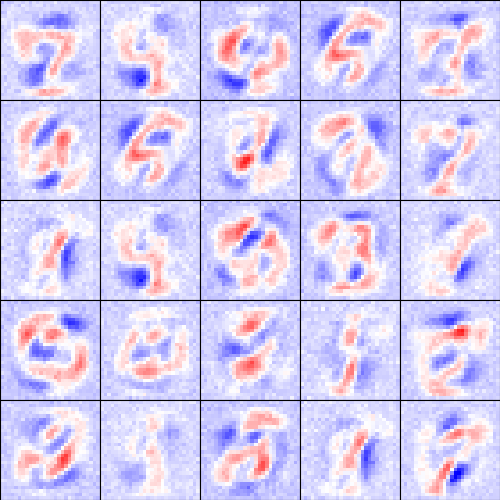
\includegraphics[width=\linewidth]{figures/rf350.iter010000.png}
   \subcaption{10000 iterations}
  \end{subfigure}
  \begin{subfigure}[b]{0.3\textwidth}
   \centering
   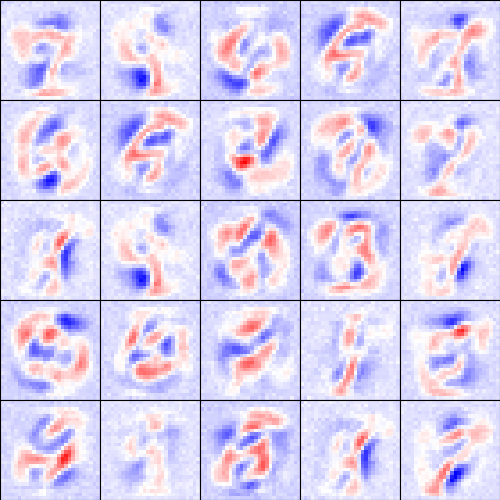
\includegraphics[width=\linewidth]{figures/rf350.iter020000.png}
   \subcaption{20000 iterations}
  \end{subfigure}
  \begin{subfigure}[b]{0.3\textwidth}
   \centering
   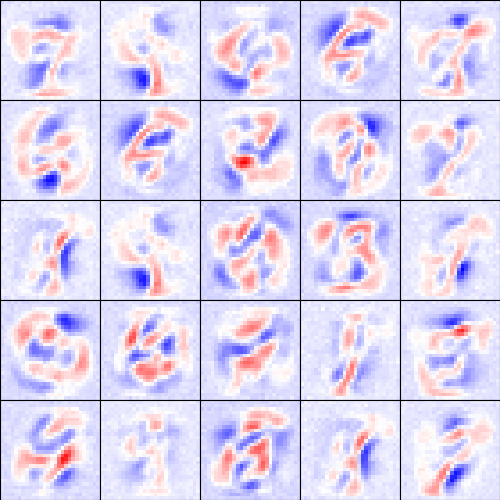
\includegraphics[width=\linewidth]{figures/rf350.iter030000.png}
   \subcaption{30000 iterations}
   \end{subfigure}
   \caption{The receptive fields in a network with 350 hidden nodes for different stages of training}
   \label{fig:receptive}
\end{figure}
\section{Deep Belief Network}
A deep belief network was formed by stacking two RBMS and concatenating a label input with the hidden layer as input for a final RBM. Greedy layer wise pre-training with CD-1 was used to train each RBM, and each hidden layer is then used as visible input layer for the next RBM in the stack. However, when using the previous layer as input for the next, the probability distributions of the RBMs become conditional and thus the weights are directed. The topmost hidden layer is never used as input for another RBM and thus retains an unconditional joint probability and undirected weights. Since the top layer is undirected, we can use Gibbs sampling to estimate and sample from the joint probability.
\subsection{Pre-training}
Each RBM was trained with 18000 training iterations, equivalent to 6 epochs using a batch size of 10. The loss function for the different layers is shown in Figure \ref{fig:layers}.The layers converge quite quickly to a almost constant loss. This could probably be improved through using better hyperparameters, although I did not really have time to do an extensive search due to computation time. The resulting DBN network is able to recognize both training and test data with about 76 \% accuracy, suggesting that there is room for a little more training. The same network can also be able to generate digits by fixing the input label and iterating for a number of times in the topmost RBM and then feeding the samples to the bottom visible layer. These generated digits are not obviously the same as the true patterns, however. A few example generated digits is shown in Figure \ref{fig:digits}.
\begin{figure}[ht]
   \centering
   \includegraphics[width=\linewidth]{figures/dbn.pdf}
   \caption{The reconstruction error over iterations for the different layers}
   \label{fig:layers}
\end{figure}
\begin{figure}[ht]
  \begin{subfigure}[b]{0.095\textwidth}
   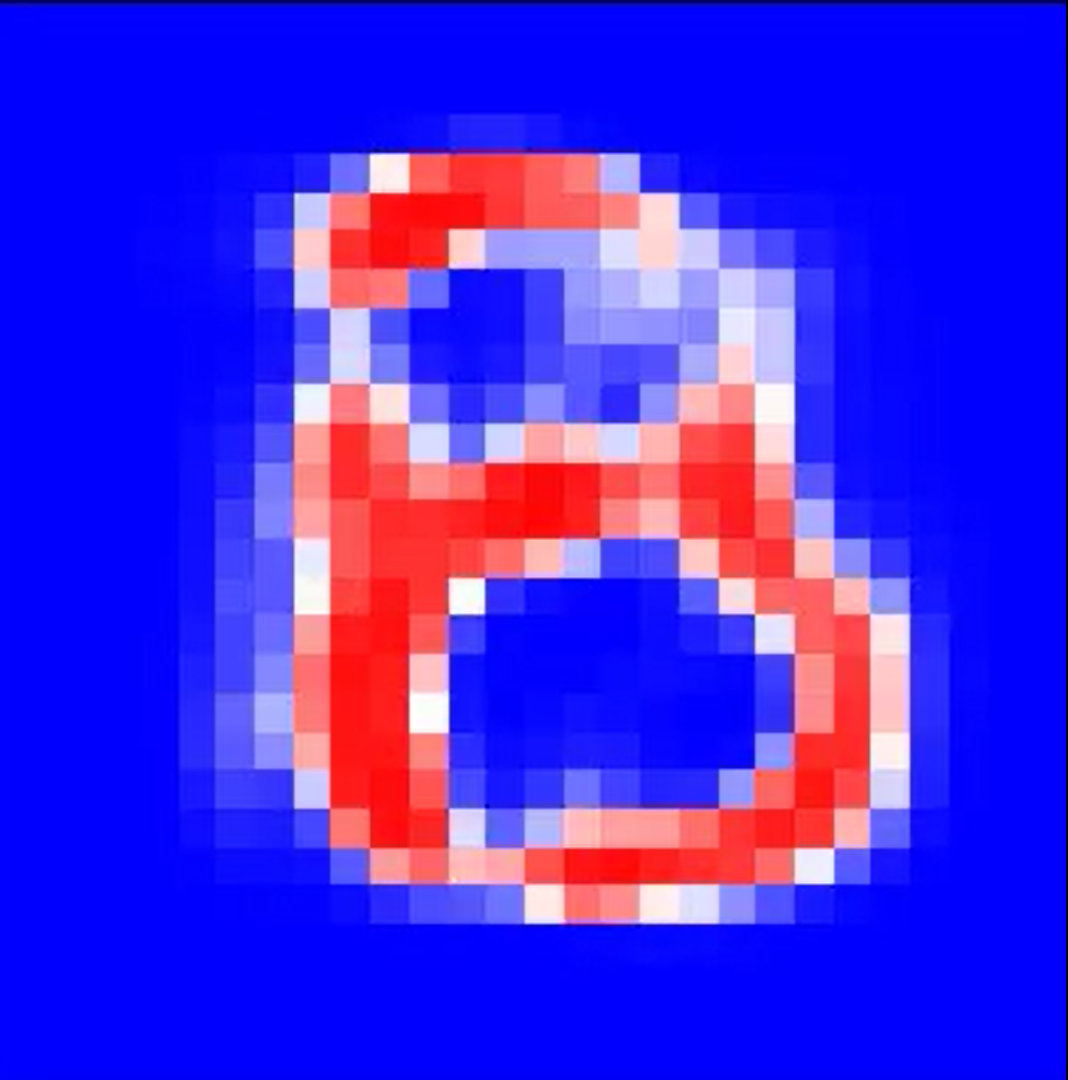
\includegraphics[width=\linewidth]{figures/0.png}
  \end{subfigure}
    \begin{subfigure}[b]{0.095\textwidth}
   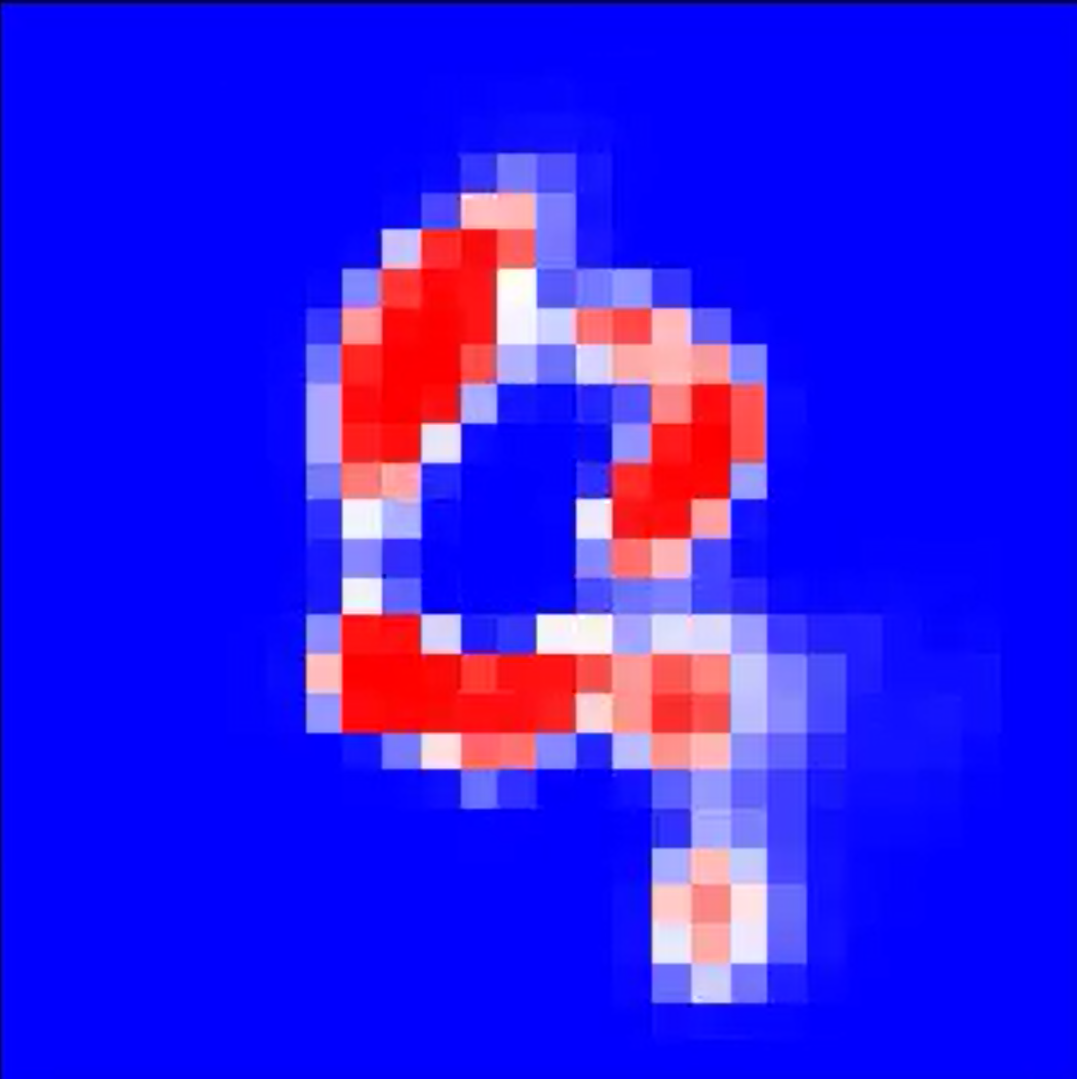
\includegraphics[width=\linewidth]{figures/1.png}
  \end{subfigure}
    \begin{subfigure}[b]{0.095\textwidth}
   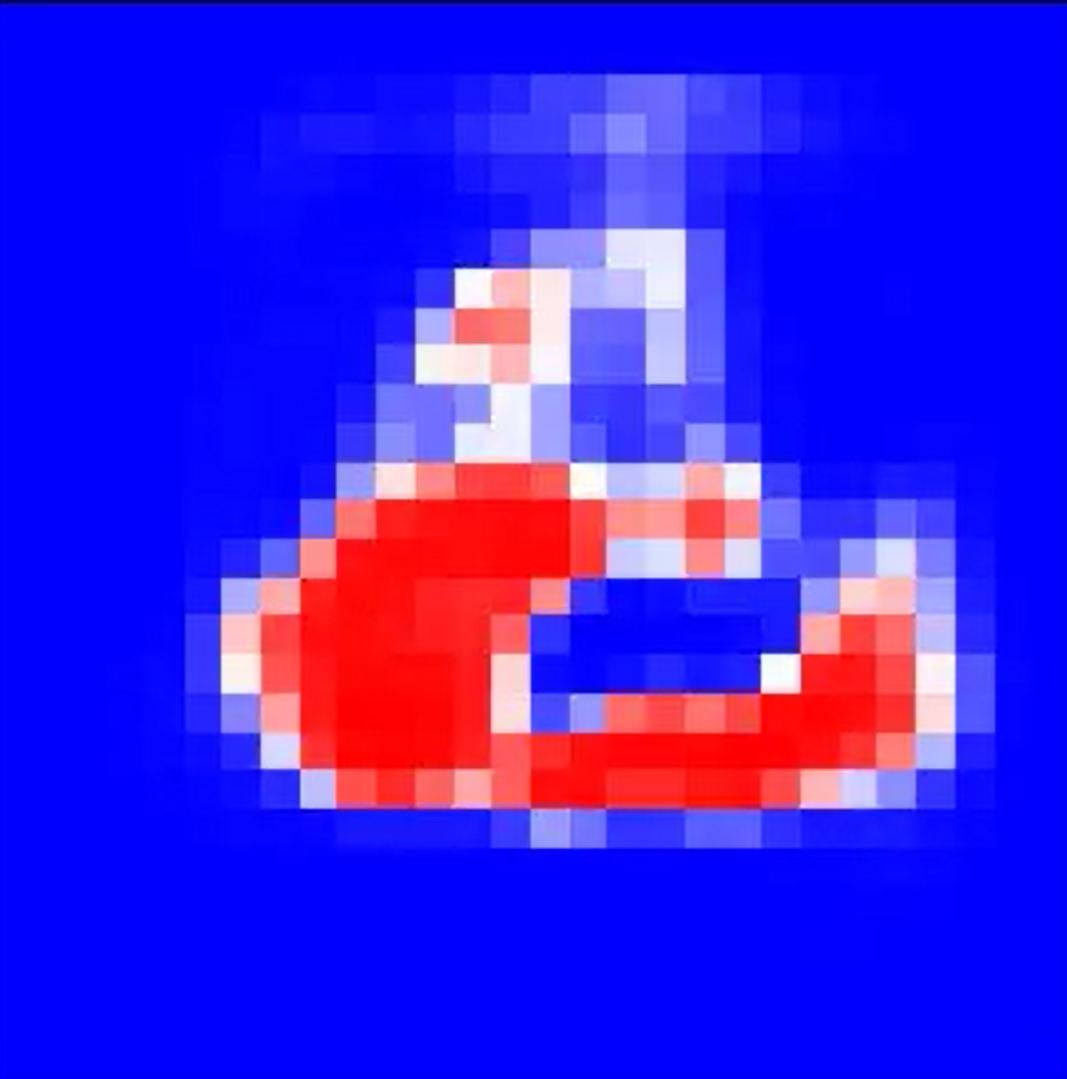
\includegraphics[width=\linewidth]{figures/2.png}
  \end{subfigure}
    \begin{subfigure}[b]{0.095\textwidth}
   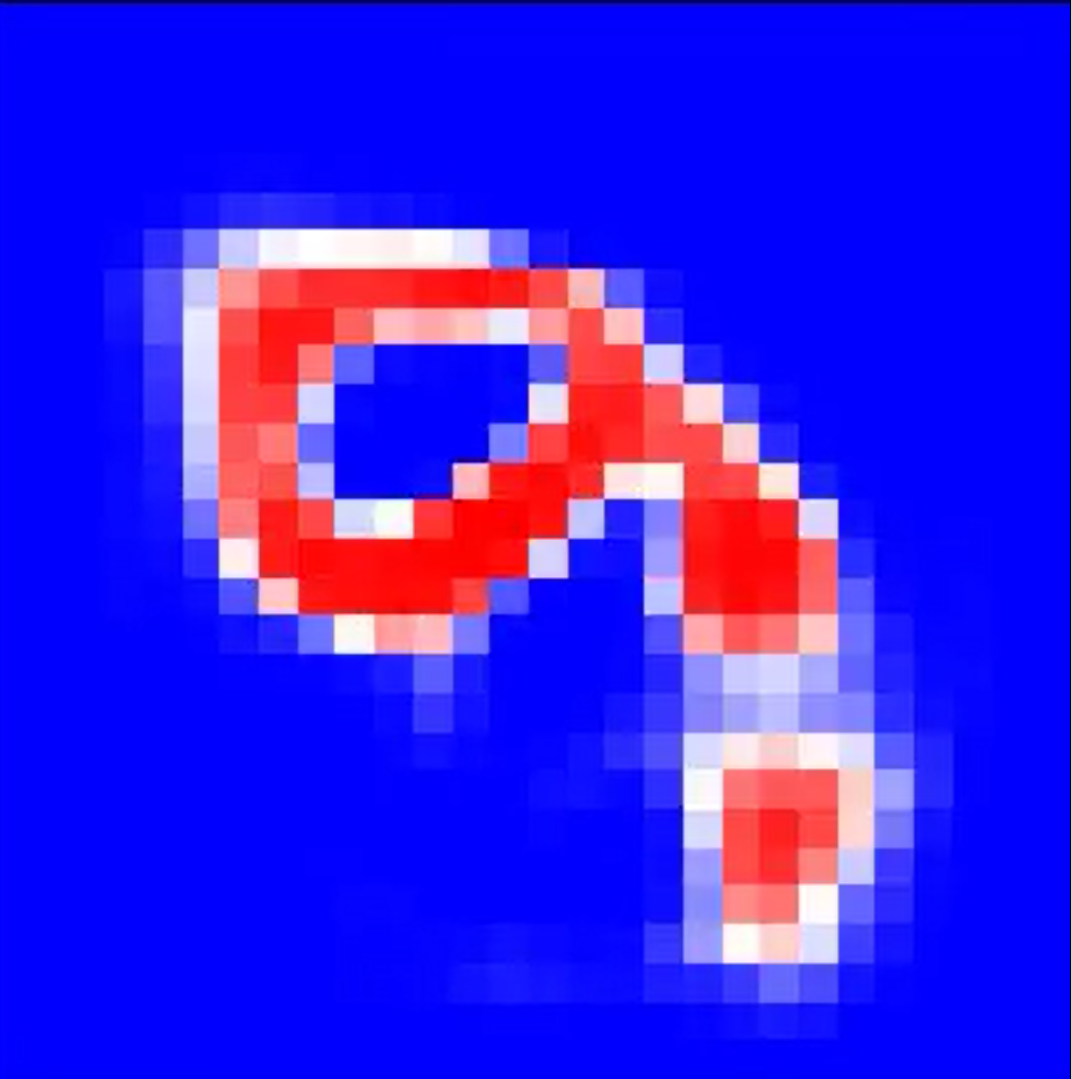
\includegraphics[width=\linewidth]{figures/3.png}
  \end{subfigure}
    \begin{subfigure}[b]{0.095\textwidth}
   
\includegraphics[width=\linewidth]{figures/4.png}
  \end{subfigure}
    \begin{subfigure}[b]{0.095\textwidth}
   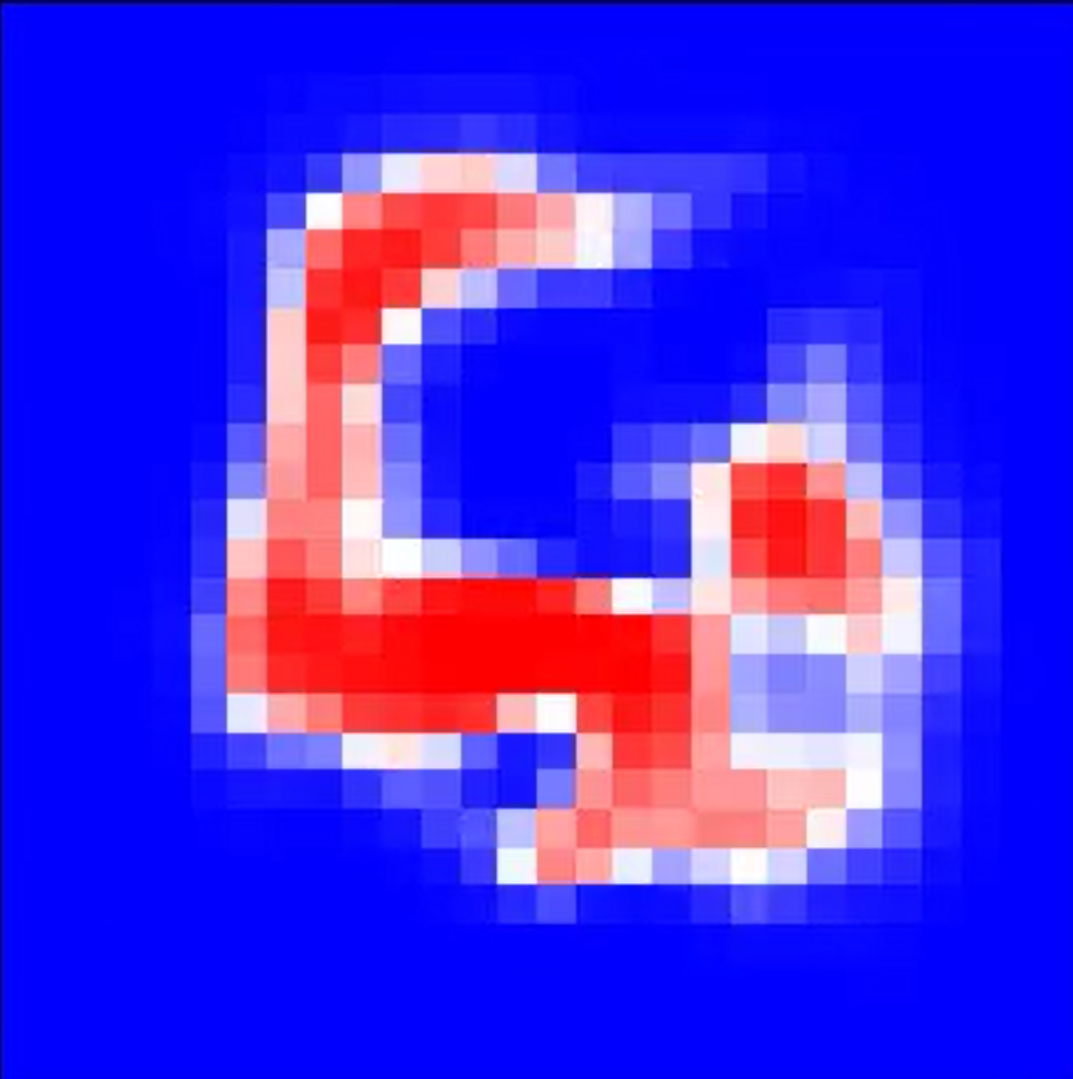
\includegraphics[width=\linewidth]{figures/5.png}
  \end{subfigure}
    \begin{subfigure}[b]{0.095\textwidth}
   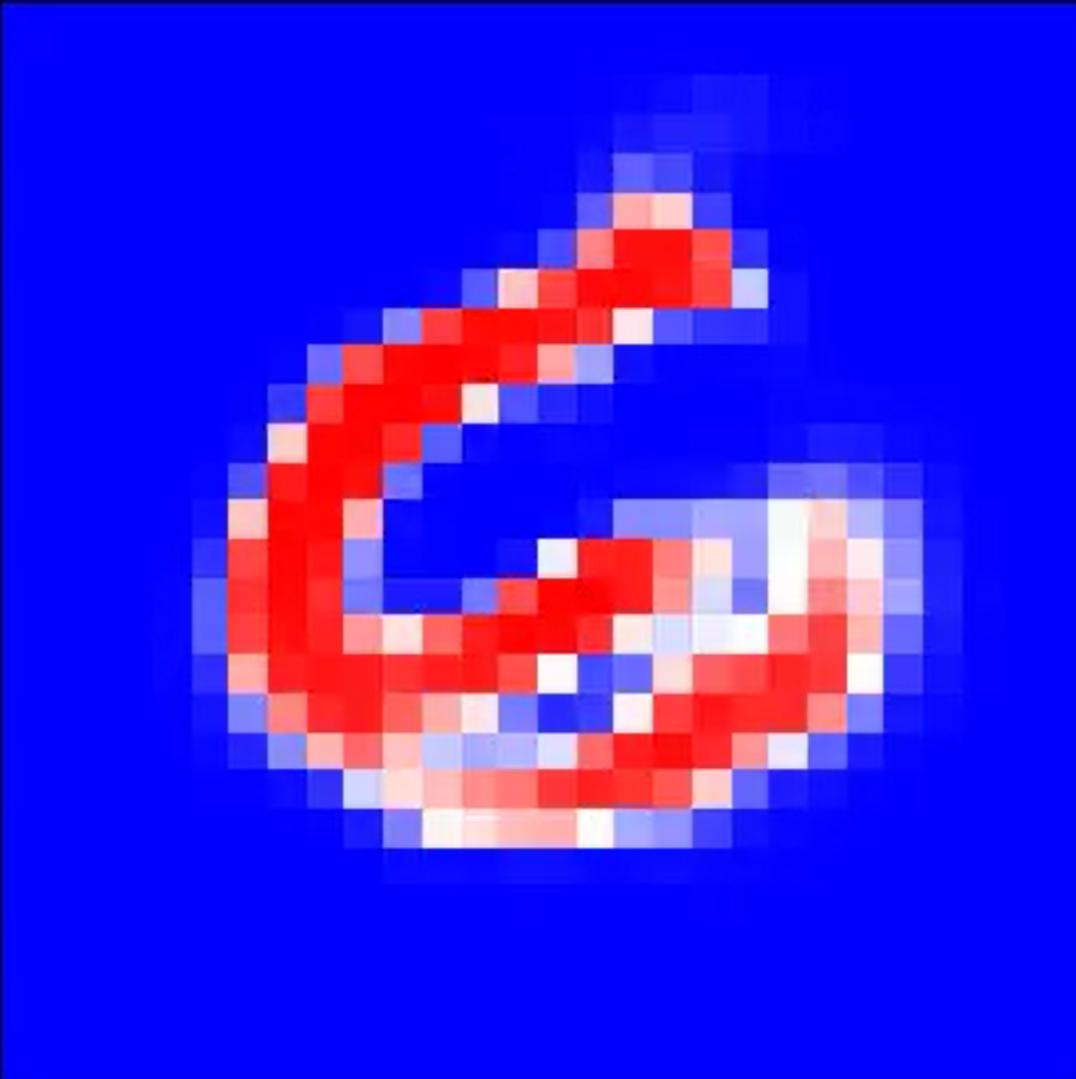
\includegraphics[width=\linewidth]{figures/6.png}
  \end{subfigure}
    \begin{subfigure}[b]{0.095\textwidth}
   
\includegraphics[width=\linewidth]{figures/7.png}
  \end{subfigure}
    \begin{subfigure}[b]{0.095\textwidth}
   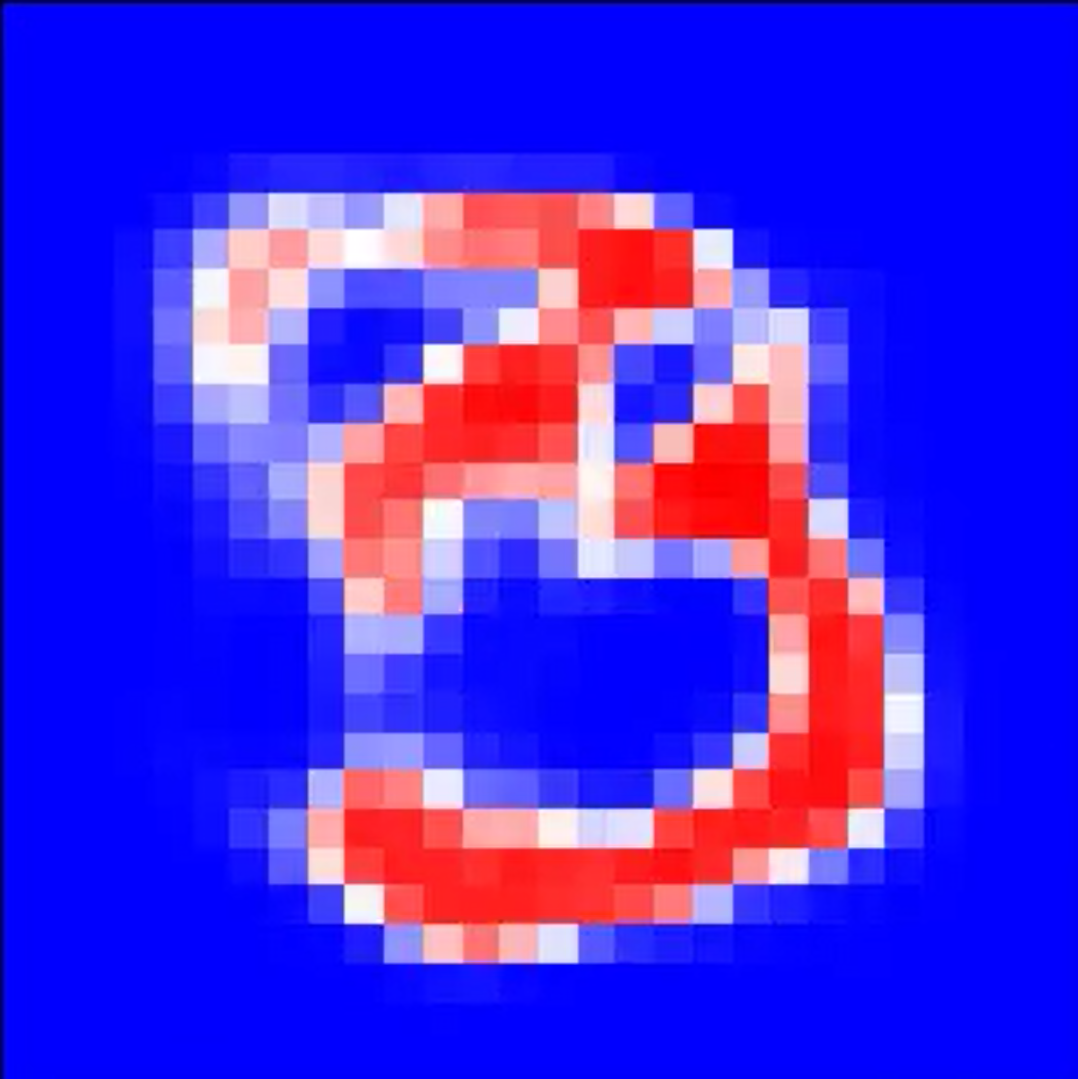
\includegraphics[width=\linewidth]{figures/8.png}
  \end{subfigure}
    \begin{subfigure}[b]{0.095\textwidth}
   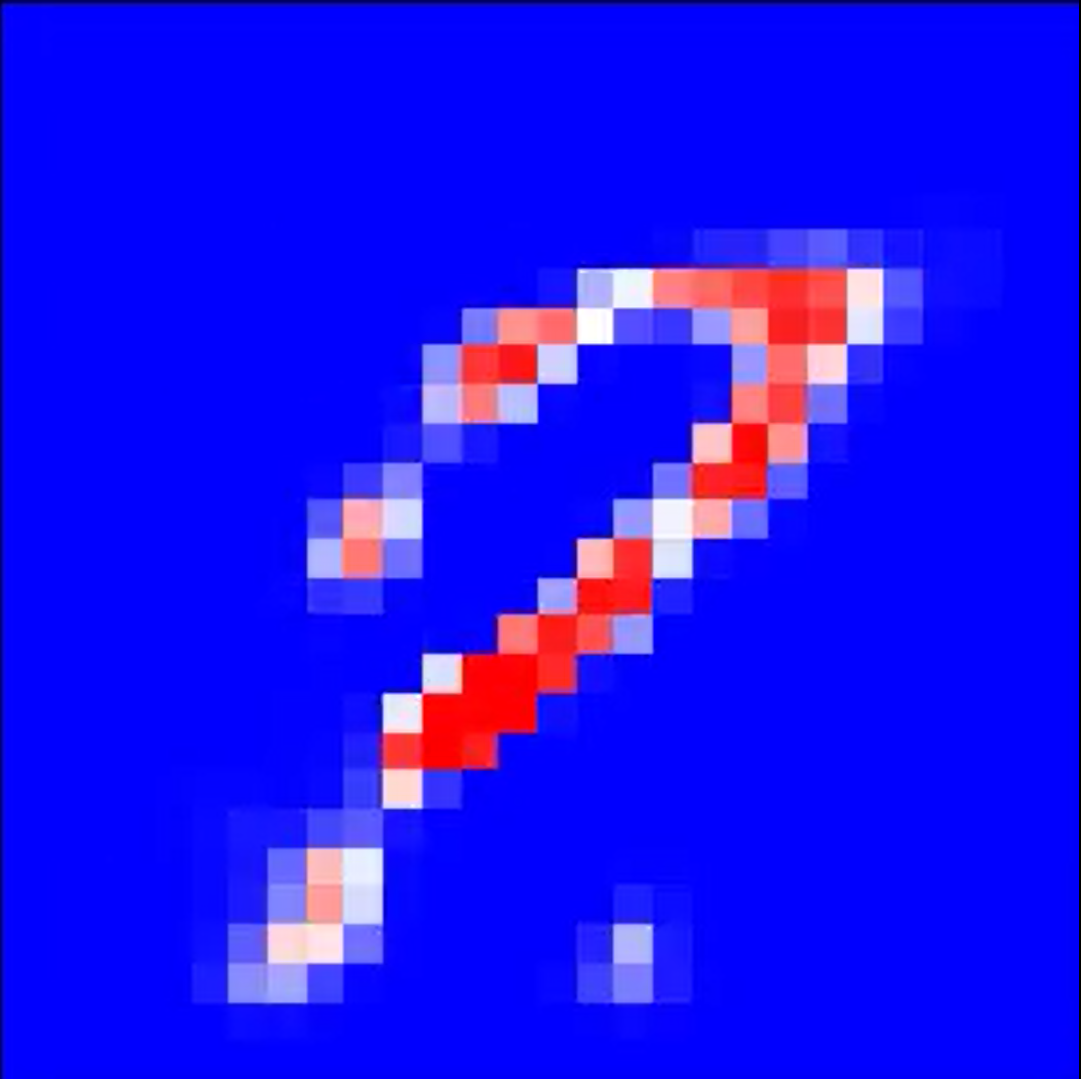
\includegraphics[width=\linewidth]{figures/9.png}
  \end{subfigure}
  \caption{The digits generated by the network}
  \label{fig:digits}
\end{figure}
\subsection{Fine-tuning}
I did not have time to finish this part.
\section{Final remarks}
Overall a very interesting lab. It was very easy to fill in the gaps from the provided code, while also aiding in the understanding. Whether to use probabilities or sampled binary numbers when updating wasn't entirely straightforward, but overall the instructions in the lab was very clear, and it was satisfying to see how "simple" archtitectures can still produce very interesting results, such as the generated receptive fields and how weight matrices can directly be mapped to something significant in 2D space. I would have liked to implement the final wake-sleep algorithm but I didn't have time.
\end{document}